

Machine learning (ML) is part of artificial intelligence (AI). as shown in Fig.~\ref{fig:ML_diagram}
AI is the process of computers being trained to mimic the human brain in how it learns and solves problems.
There are two types of learning: ML learning where it needs human intervene, and deep learning (DL) which is a subset of ML where computers learn from its own errors.  

ML is algorithms, collection of tools and techniques, with the ability to learn without being explicitly programmed, more data better decisions.

ML algor could be categorized into two main groups depending on the data used in training the machine learning model: supervised learning, using labeled data (target) and unsupervised learning.

There are dozens of different ML methods (algorithms) that could be used depending on the problem we want to solve either to classify things (classification problem) or make quantitative predictions (regression problem).
Both of these problems are supervised leaning.

ML model is the result of running a ML algorithm on data. It contains the model data and prediction algorithm. 

Various python-based libraries such as schitkit-learn, TensorFlow, keras are used tools for ML algorithms and model implementation.  

\begin{figure}[t!]
\centering
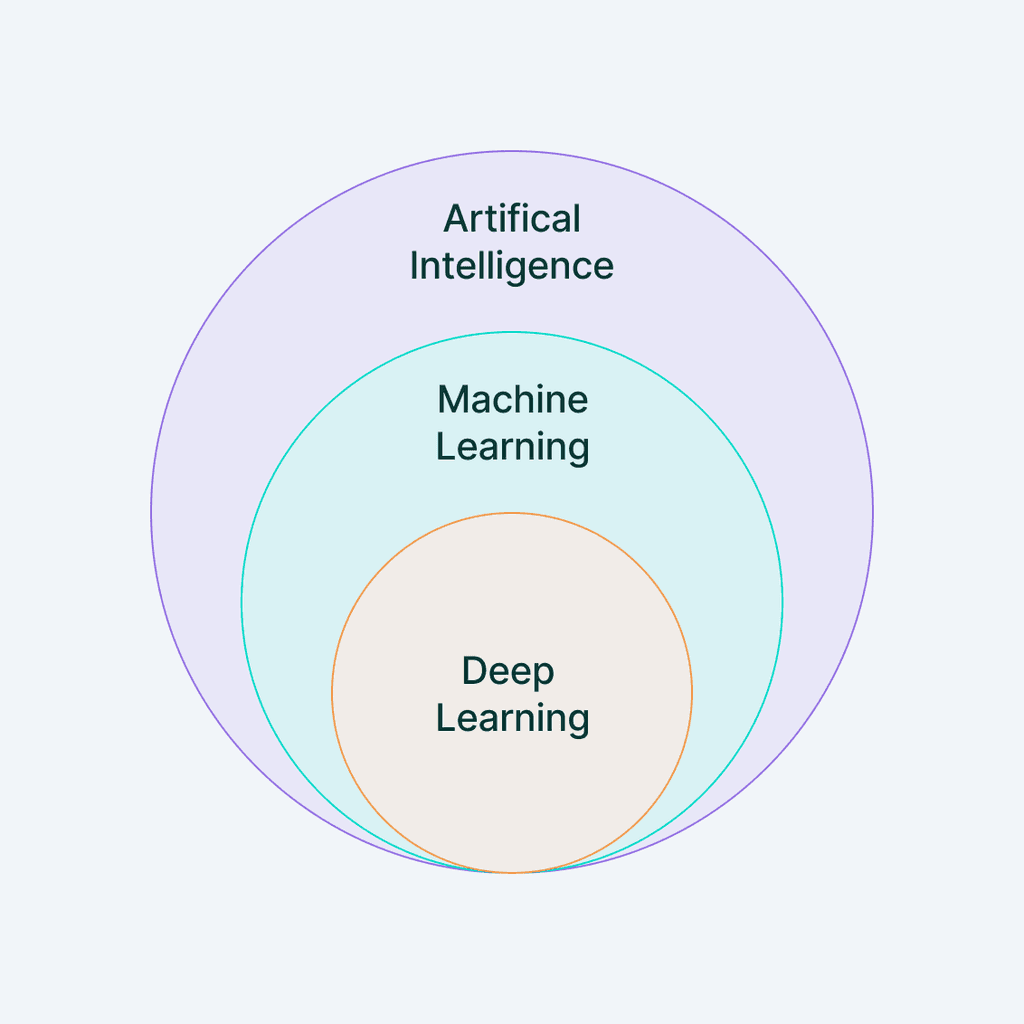
\includegraphics[width=0.99\textwidth]{figures/ML_diagram.png}
\caption[ML and AI]{}. Figure source~\cite{SMtable}.
\label{fig:ML_diagram}}                                                                                                                                                                                        
\end{figure}
  
%% .....  previous draft .....  % 
%machine learning is a collection of tools and techniques that transforms data.

%ML could be use to classify things (this known as classification)
%or make quantitative predictions (regression).

%(in this thesis ML are used for regression)

%(note: there are a lot of ML methods to choose from. how can we pick the best one for our problem?)

%In general to choose the best ML method that fit our problem,
%we can compare the prediction of each method with the true value to see how well each method performs.

%In ML we could split out data into two group:
%training data (where the ML method will learn to make prediction. in other words fit the data),
%testing data (used to compare predictions made by different ML methods. in other words used to evaluate the ML method) )

%In testing we can measure the error (distance between the prediction and observed (true) value).
%meaning we are going to compare the sum of the errors.
%the shorter the error the better the model at making predictions. 

%Types of vaiables:
%the independent varaible (feature) is used by the ML method in making predictions.
%dependent variable (target) is the varaible predicted by ML method.

%Very comman to use multiple features to make predictions.

% source ch1.

%models (probability distrubtion, approximate a historgram) or equations (approximate a relationship between varaibles)

%usually approximate relatiy to let us explore relationships and make predictions.

%In ML we build models by training ML algorithms with training data.

%we use statistics to determine of a model is useful or believable. 

%% The goal of ML method here is to learn from "training data" to make predictions.  
%% source: statequest
%................................................................................



